\documentclass[twoside]{book}

% Packages required by doxygen
\usepackage{fixltx2e}
\usepackage{calc}
\usepackage{doxygen}
\usepackage[export]{adjustbox} % also loads graphicx
\usepackage{graphicx}
\usepackage[utf8]{inputenc}
\usepackage{makeidx}
\usepackage{multicol}
\usepackage{multirow}
\PassOptionsToPackage{warn}{textcomp}
\usepackage{textcomp}
\usepackage[nointegrals]{wasysym}
\usepackage[table]{xcolor}

% Font selection
\usepackage[T1]{fontenc}
\usepackage[scaled=.90]{helvet}
\usepackage{courier}
\usepackage{amssymb}
\usepackage{sectsty}
\renewcommand{\familydefault}{\sfdefault}
\allsectionsfont{%
  \fontseries{bc}\selectfont%
  \color{darkgray}%
}
\renewcommand{\DoxyLabelFont}{%
  \fontseries{bc}\selectfont%
  \color{darkgray}%
}
\newcommand{\+}{\discretionary{\mbox{\scriptsize$\hookleftarrow$}}{}{}}

% Page & text layout
\usepackage{geometry}
\geometry{%
  a4paper,%
  top=2.5cm,%
  bottom=2.5cm,%
  left=2.5cm,%
  right=2.5cm%
}
\tolerance=750
\hfuzz=15pt
\hbadness=750
\setlength{\emergencystretch}{15pt}
\setlength{\parindent}{0cm}
\setlength{\parskip}{3ex plus 2ex minus 2ex}
\makeatletter
\renewcommand{\paragraph}{%
  \@startsection{paragraph}{4}{0ex}{-1.0ex}{1.0ex}{%
    \normalfont\normalsize\bfseries\SS@parafont%
  }%
}
\renewcommand{\subparagraph}{%
  \@startsection{subparagraph}{5}{0ex}{-1.0ex}{1.0ex}{%
    \normalfont\normalsize\bfseries\SS@subparafont%
  }%
}
\makeatother

% Headers & footers
\usepackage{fancyhdr}
\pagestyle{fancyplain}
\fancyhead[LE]{\fancyplain{}{\bfseries\thepage}}
\fancyhead[CE]{\fancyplain{}{}}
\fancyhead[RE]{\fancyplain{}{\bfseries\leftmark}}
\fancyhead[LO]{\fancyplain{}{\bfseries\rightmark}}
\fancyhead[CO]{\fancyplain{}{}}
\fancyhead[RO]{\fancyplain{}{\bfseries\thepage}}
\fancyfoot[LE]{\fancyplain{}{}}
\fancyfoot[CE]{\fancyplain{}{}}
\fancyfoot[RE]{\fancyplain{}{\bfseries\scriptsize Generated by Doxygen }}
\fancyfoot[LO]{\fancyplain{}{\bfseries\scriptsize Generated by Doxygen }}
\fancyfoot[CO]{\fancyplain{}{}}
\fancyfoot[RO]{\fancyplain{}{}}
\renewcommand{\footrulewidth}{0.4pt}
\renewcommand{\chaptermark}[1]{%
  \markboth{#1}{}%
}
\renewcommand{\sectionmark}[1]{%
  \markright{\thesection\ #1}%
}

% Indices & bibliography
\usepackage{natbib}
\usepackage[titles]{tocloft}
\setcounter{tocdepth}{3}
\setcounter{secnumdepth}{5}
\makeindex

% Hyperlinks (required, but should be loaded last)
\usepackage{ifpdf}
\ifpdf
  \usepackage[pdftex,pagebackref=true]{hyperref}
\else
  \usepackage[ps2pdf,pagebackref=true]{hyperref}
\fi
\hypersetup{%
  colorlinks=true,%
  linkcolor=blue,%
  citecolor=blue,%
  unicode%
}

% Custom commands
\newcommand{\clearemptydoublepage}{%
  \newpage{\pagestyle{empty}\cleardoublepage}%
}

\usepackage{caption}
\captionsetup{labelsep=space,justification=centering,font={bf},singlelinecheck=off,skip=4pt,position=top}

%===== C O N T E N T S =====

\begin{document}

% Titlepage & ToC
\hypersetup{pageanchor=false,
             bookmarksnumbered=true,
             pdfencoding=unicode
            }
\pagenumbering{alph}
\begin{titlepage}
\vspace*{7cm}
\begin{center}%
{\Large U\+DP server connection \\[1ex]\large 1 }\\
\vspace*{1cm}
{\large Generated by Doxygen 1.8.13}\\
\end{center}
\end{titlepage}
\clearemptydoublepage
\pagenumbering{roman}
\tableofcontents
\clearemptydoublepage
\pagenumbering{arabic}
\hypersetup{pageanchor=true}

%--- Begin generated contents ---
\chapter{Namespace Index}
\section{Namespace List}
Here is a list of all namespaces with brief descriptions\+:\begin{DoxyCompactList}
\item\contentsline{section}{\hyperlink{namespaceudp__client__server}{udp\+\_\+client\+\_\+server} }{\pageref{namespaceudp__client__server}}{}
\end{DoxyCompactList}

\chapter{File Index}
\section{File List}
Here is a list of all files with brief descriptions\+:\begin{DoxyCompactList}
\item\contentsline{section}{D\+:/cloned repo trainawear/train-\/\+A-\/wear/\+Phone App/app/build/generated/not\+\_\+namespaced\+\_\+r\+\_\+class\+\_\+sources/debug/process\+Debug\+Resources/r/android/arch/core/\mbox{\hyperlink{process_debug_resources_2r_2android_2arch_2core_2_r_8java}{R.\+java}} }{\pageref{process_debug_resources_2r_2android_2arch_2core_2_r_8java}}{}
\item\contentsline{section}{D\+:/cloned repo trainawear/train-\/\+A-\/wear/\+Phone App/app/build/generated/not\+\_\+namespaced\+\_\+r\+\_\+class\+\_\+sources/debug/process\+Debug\+Resources/r/android/arch/lifecycle/\mbox{\hyperlink{process_debug_resources_2r_2android_2arch_2lifecycle_2_r_8java}{R.\+java}} }{\pageref{process_debug_resources_2r_2android_2arch_2lifecycle_2_r_8java}}{}
\item\contentsline{section}{D\+:/cloned repo trainawear/train-\/\+A-\/wear/\+Phone App/app/build/generated/not\+\_\+namespaced\+\_\+r\+\_\+class\+\_\+sources/debug/process\+Debug\+Resources/r/android/arch/lifecycle/livedata/core/\mbox{\hyperlink{process_debug_resources_2r_2android_2arch_2lifecycle_2livedata_2core_2_r_8java}{R.\+java}} }{\pageref{process_debug_resources_2r_2android_2arch_2lifecycle_2livedata_2core_2_r_8java}}{}
\item\contentsline{section}{D\+:/cloned repo trainawear/train-\/\+A-\/wear/\+Phone App/app/build/generated/not\+\_\+namespaced\+\_\+r\+\_\+class\+\_\+sources/debug/process\+Debug\+Resources/r/android/arch/lifecycle/viewmodel/\mbox{\hyperlink{process_debug_resources_2r_2android_2arch_2lifecycle_2viewmodel_2_r_8java}{R.\+java}} }{\pageref{process_debug_resources_2r_2android_2arch_2lifecycle_2viewmodel_2_r_8java}}{}
\item\contentsline{section}{D\+:/cloned repo trainawear/train-\/\+A-\/wear/\+Phone App/app/build/generated/not\+\_\+namespaced\+\_\+r\+\_\+class\+\_\+sources/debug/process\+Debug\+Resources/r/android/support/compat/\mbox{\hyperlink{process_debug_resources_2r_2android_2support_2compat_2_r_8java}{R.\+java}} }{\pageref{process_debug_resources_2r_2android_2support_2compat_2_r_8java}}{}
\item\contentsline{section}{D\+:/cloned repo trainawear/train-\/\+A-\/wear/\+Phone App/app/build/generated/not\+\_\+namespaced\+\_\+r\+\_\+class\+\_\+sources/debug/process\+Debug\+Resources/r/android/support/constraint/\mbox{\hyperlink{process_debug_resources_2r_2android_2support_2constraint_2_r_8java}{R.\+java}} }{\pageref{process_debug_resources_2r_2android_2support_2constraint_2_r_8java}}{}
\item\contentsline{section}{D\+:/cloned repo trainawear/train-\/\+A-\/wear/\+Phone App/app/build/generated/not\+\_\+namespaced\+\_\+r\+\_\+class\+\_\+sources/debug/process\+Debug\+Resources/r/android/support/coreui/\mbox{\hyperlink{process_debug_resources_2r_2android_2support_2coreui_2_r_8java}{R.\+java}} }{\pageref{process_debug_resources_2r_2android_2support_2coreui_2_r_8java}}{}
\item\contentsline{section}{D\+:/cloned repo trainawear/train-\/\+A-\/wear/\+Phone App/app/build/generated/not\+\_\+namespaced\+\_\+r\+\_\+class\+\_\+sources/debug/process\+Debug\+Resources/r/android/support/coreutils/\mbox{\hyperlink{process_debug_resources_2r_2android_2support_2coreutils_2_r_8java}{R.\+java}} }{\pageref{process_debug_resources_2r_2android_2support_2coreutils_2_r_8java}}{}
\item\contentsline{section}{D\+:/cloned repo trainawear/train-\/\+A-\/wear/\+Phone App/app/build/generated/not\+\_\+namespaced\+\_\+r\+\_\+class\+\_\+sources/debug/process\+Debug\+Resources/r/android/support/design/\mbox{\hyperlink{process_debug_resources_2r_2android_2support_2design_2_r_8java}{R.\+java}} }{\pageref{process_debug_resources_2r_2android_2support_2design_2_r_8java}}{}
\item\contentsline{section}{D\+:/cloned repo trainawear/train-\/\+A-\/wear/\+Phone App/app/build/generated/not\+\_\+namespaced\+\_\+r\+\_\+class\+\_\+sources/debug/process\+Debug\+Resources/r/android/support/fragment/\mbox{\hyperlink{process_debug_resources_2r_2android_2support_2fragment_2_r_8java}{R.\+java}} }{\pageref{process_debug_resources_2r_2android_2support_2fragment_2_r_8java}}{}
\item\contentsline{section}{D\+:/cloned repo trainawear/train-\/\+A-\/wear/\+Phone App/app/build/generated/not\+\_\+namespaced\+\_\+r\+\_\+class\+\_\+sources/debug/process\+Debug\+Resources/r/android/support/graphics/drawable/\mbox{\hyperlink{process_debug_resources_2r_2android_2support_2graphics_2drawable_2_r_8java}{R.\+java}} }{\pageref{process_debug_resources_2r_2android_2support_2graphics_2drawable_2_r_8java}}{}
\item\contentsline{section}{D\+:/cloned repo trainawear/train-\/\+A-\/wear/\+Phone App/app/build/generated/not\+\_\+namespaced\+\_\+r\+\_\+class\+\_\+sources/debug/process\+Debug\+Resources/r/android/support/graphics/drawable/animated/\mbox{\hyperlink{process_debug_resources_2r_2android_2support_2graphics_2drawable_2animated_2_r_8java}{R.\+java}} }{\pageref{process_debug_resources_2r_2android_2support_2graphics_2drawable_2animated_2_r_8java}}{}
\item\contentsline{section}{D\+:/cloned repo trainawear/train-\/\+A-\/wear/\+Phone App/app/build/generated/not\+\_\+namespaced\+\_\+r\+\_\+class\+\_\+sources/debug/process\+Debug\+Resources/r/android/support/mediacompat/\mbox{\hyperlink{process_debug_resources_2r_2android_2support_2mediacompat_2_r_8java}{R.\+java}} }{\pageref{process_debug_resources_2r_2android_2support_2mediacompat_2_r_8java}}{}
\item\contentsline{section}{D\+:/cloned repo trainawear/train-\/\+A-\/wear/\+Phone App/app/build/generated/not\+\_\+namespaced\+\_\+r\+\_\+class\+\_\+sources/debug/process\+Debug\+Resources/r/android/support/transition/\mbox{\hyperlink{process_debug_resources_2r_2android_2support_2transition_2_r_8java}{R.\+java}} }{\pageref{process_debug_resources_2r_2android_2support_2transition_2_r_8java}}{}
\item\contentsline{section}{D\+:/cloned repo trainawear/train-\/\+A-\/wear/\+Phone App/app/build/generated/not\+\_\+namespaced\+\_\+r\+\_\+class\+\_\+sources/debug/process\+Debug\+Resources/r/android/support/v4/\mbox{\hyperlink{process_debug_resources_2r_2android_2support_2v4_2_r_8java}{R.\+java}} }{\pageref{process_debug_resources_2r_2android_2support_2v4_2_r_8java}}{}
\item\contentsline{section}{D\+:/cloned repo trainawear/train-\/\+A-\/wear/\+Phone App/app/build/generated/not\+\_\+namespaced\+\_\+r\+\_\+class\+\_\+sources/debug/process\+Debug\+Resources/r/android/support/v7/appcompat/\mbox{\hyperlink{process_debug_resources_2r_2android_2support_2v7_2appcompat_2_r_8java}{R.\+java}} }{\pageref{process_debug_resources_2r_2android_2support_2v7_2appcompat_2_r_8java}}{}
\item\contentsline{section}{D\+:/cloned repo trainawear/train-\/\+A-\/wear/\+Phone App/app/build/generated/not\+\_\+namespaced\+\_\+r\+\_\+class\+\_\+sources/debug/process\+Debug\+Resources/r/android/support/v7/recyclerview/\mbox{\hyperlink{process_debug_resources_2r_2android_2support_2v7_2recyclerview_2_r_8java}{R.\+java}} }{\pageref{process_debug_resources_2r_2android_2support_2v7_2recyclerview_2_r_8java}}{}
\item\contentsline{section}{D\+:/cloned repo trainawear/train-\/\+A-\/wear/\+Phone App/app/build/generated/not\+\_\+namespaced\+\_\+r\+\_\+class\+\_\+sources/debug/process\+Debug\+Resources/r/com/example/trainawearapplication/\mbox{\hyperlink{process_debug_resources_2r_2com_2example_2trainawearapplication_2_r_8java}{R.\+java}} }{\pageref{process_debug_resources_2r_2com_2example_2trainawearapplication_2_r_8java}}{}
\item\contentsline{section}{D\+:/cloned repo trainawear/train-\/\+A-\/wear/\+Phone App/app/build/generated/not\+\_\+namespaced\+\_\+r\+\_\+class\+\_\+sources/debug/process\+Debug\+Resources/r/com/jjoe64/graphview/\mbox{\hyperlink{process_debug_resources_2r_2com_2jjoe64_2graphview_2_r_8java}{R.\+java}} }{\pageref{process_debug_resources_2r_2com_2jjoe64_2graphview_2_r_8java}}{}
\item\contentsline{section}{D\+:/cloned repo trainawear/train-\/\+A-\/wear/\+Phone App/app/build/generated/not\+\_\+namespaced\+\_\+r\+\_\+class\+\_\+sources/debug/process\+Debug\+Resources/r/com/synnapps/carouselview/\mbox{\hyperlink{process_debug_resources_2r_2com_2synnapps_2carouselview_2_r_8java}{R.\+java}} }{\pageref{process_debug_resources_2r_2com_2synnapps_2carouselview_2_r_8java}}{}
\item\contentsline{section}{D\+:/cloned repo trainawear/train-\/\+A-\/wear/\+Phone App/app/build/generated/not\+\_\+namespaced\+\_\+r\+\_\+class\+\_\+sources/debug\+Android\+Test/process\+Debug\+Android\+Test\+Resources/r/android/support/test/\mbox{\hyperlink{ndroid_test_2process_debug_android_test_resources_2r_2android_2support_2test_2_r_8java}{R.\+java}} }{\pageref{ndroid_test_2process_debug_android_test_resources_2r_2android_2support_2test_2_r_8java}}{}
\item\contentsline{section}{D\+:/cloned repo trainawear/train-\/\+A-\/wear/\+Phone App/app/build/generated/not\+\_\+namespaced\+\_\+r\+\_\+class\+\_\+sources/debug\+Android\+Test/process\+Debug\+Android\+Test\+Resources/r/android/support/test/espresso/\mbox{\hyperlink{ndroid_test_2process_debug_android_test_resources_2r_2android_2support_2test_2espresso_2_r_8java}{R.\+java}} }{\pageref{ndroid_test_2process_debug_android_test_resources_2r_2android_2support_2test_2espresso_2_r_8java}}{}
\item\contentsline{section}{D\+:/cloned repo trainawear/train-\/\+A-\/wear/\+Phone App/app/build/generated/not\+\_\+namespaced\+\_\+r\+\_\+class\+\_\+sources/debug\+Android\+Test/process\+Debug\+Android\+Test\+Resources/r/com/example/trainawearapplication/test/\mbox{\hyperlink{ndroid_test_2process_debug_android_test_resources_2r_2com_2example_2trainawearapplication_2test_2_r_8java}{R.\+java}} }{\pageref{ndroid_test_2process_debug_android_test_resources_2r_2com_2example_2trainawearapplication_2test_2_r_8java}}{}
\item\contentsline{section}{D\+:/cloned repo trainawear/train-\/\+A-\/wear/\+Phone App/app/build/generated/source/build\+Config/android\+Test/debug/com/example/trainawearapplication/test/\mbox{\hyperlink{android_test_2debug_2com_2example_2trainawearapplication_2test_2_build_config_8java}{Build\+Config.\+java}} }{\pageref{android_test_2debug_2com_2example_2trainawearapplication_2test_2_build_config_8java}}{}
\item\contentsline{section}{D\+:/cloned repo trainawear/train-\/\+A-\/wear/\+Phone App/app/build/generated/source/build\+Config/debug/com/example/trainawearapplication/\mbox{\hyperlink{debug_2com_2example_2trainawearapplication_2_build_config_8java}{Build\+Config.\+java}} }{\pageref{debug_2com_2example_2trainawearapplication_2_build_config_8java}}{}
\item\contentsline{section}{D\+:/cloned repo trainawear/train-\/\+A-\/wear/\+Phone App/app/src/android\+Test/java/com/example/trainawearapplication/\mbox{\hyperlink{_example_instrumented_test_8java}{Example\+Instrumented\+Test.\+java}} }{\pageref{_example_instrumented_test_8java}}{}
\item\contentsline{section}{D\+:/cloned repo trainawear/train-\/\+A-\/wear/\+Phone App/app/src/android\+Test/java/com/example/trainawearapplication/\mbox{\hyperlink{_setup_instrumentation_test_8java}{Setup\+Instrumentation\+Test.\+java}} }{\pageref{_setup_instrumentation_test_8java}}{}
\item\contentsline{section}{D\+:/cloned repo trainawear/train-\/\+A-\/wear/\+Phone App/app/src/main/java/com/example/trainawearapplication/\mbox{\hyperlink{_biceps_8java}{Biceps.\+java}} }{\pageref{_biceps_8java}}{}
\item\contentsline{section}{D\+:/cloned repo trainawear/train-\/\+A-\/wear/\+Phone App/app/src/main/java/com/example/trainawearapplication/\mbox{\hyperlink{_classic_squat_8java}{Classic\+Squat.\+java}} }{\pageref{_classic_squat_8java}}{}
\item\contentsline{section}{D\+:/cloned repo trainawear/train-\/\+A-\/wear/\+Phone App/app/src/main/java/com/example/trainawearapplication/\mbox{\hyperlink{_client_listen_8java}{Client\+Listen.\+java}} }{\pageref{_client_listen_8java}}{}
\item\contentsline{section}{D\+:/cloned repo trainawear/train-\/\+A-\/wear/\+Phone App/app/src/main/java/com/example/trainawearapplication/\mbox{\hyperlink{_client_listen_bicep_8java}{Client\+Listen\+Bicep.\+java}} }{\pageref{_client_listen_bicep_8java}}{}
\item\contentsline{section}{D\+:/cloned repo trainawear/train-\/\+A-\/wear/\+Phone App/app/src/main/java/com/example/trainawearapplication/\mbox{\hyperlink{_client_listen_plank_8java}{Client\+Listen\+Plank.\+java}} }{\pageref{_client_listen_plank_8java}}{}
\item\contentsline{section}{D\+:/cloned repo trainawear/train-\/\+A-\/wear/\+Phone App/app/src/main/java/com/example/trainawearapplication/\mbox{\hyperlink{_client_send_8java}{Client\+Send.\+java}} }{\pageref{_client_send_8java}}{}
\item\contentsline{section}{D\+:/cloned repo trainawear/train-\/\+A-\/wear/\+Phone App/app/src/main/java/com/example/trainawearapplication/\mbox{\hyperlink{_help_app_8java}{Help\+App.\+java}} }{\pageref{_help_app_8java}}{}
\item\contentsline{section}{D\+:/cloned repo trainawear/train-\/\+A-\/wear/\+Phone App/app/src/main/java/com/example/trainawearapplication/\mbox{\hyperlink{_main_activity_8java}{Main\+Activity.\+java}} }{\pageref{_main_activity_8java}}{}
\item\contentsline{section}{D\+:/cloned repo trainawear/train-\/\+A-\/wear/\+Phone App/app/src/main/java/com/example/trainawearapplication/\mbox{\hyperlink{_modified_scroll_view_8java}{Modified\+Scroll\+View.\+java}} }{\pageref{_modified_scroll_view_8java}}{}
\item\contentsline{section}{D\+:/cloned repo trainawear/train-\/\+A-\/wear/\+Phone App/app/src/main/java/com/example/trainawearapplication/\mbox{\hyperlink{_plank_8java}{Plank.\+java}} }{\pageref{_plank_8java}}{}
\item\contentsline{section}{D\+:/cloned repo trainawear/train-\/\+A-\/wear/\+Phone App/app/src/main/java/com/example/trainawearapplication/\mbox{\hyperlink{_plie_squat_8java}{Plie\+Squat.\+java}} }{\pageref{_plie_squat_8java}}{}
\item\contentsline{section}{D\+:/cloned repo trainawear/train-\/\+A-\/wear/\+Phone App/app/src/main/java/com/example/trainawearapplication/\mbox{\hyperlink{_progress_8java}{Progress.\+java}} }{\pageref{_progress_8java}}{}
\item\contentsline{section}{D\+:/cloned repo trainawear/train-\/\+A-\/wear/\+Phone App/app/src/main/java/com/example/trainawearapplication/\mbox{\hyperlink{_setup_8java}{Setup.\+java}} }{\pageref{_setup_8java}}{}
\item\contentsline{section}{D\+:/cloned repo trainawear/train-\/\+A-\/wear/\+Phone App/app/src/main/java/com/example/trainawearapplication/\mbox{\hyperlink{_squat_8java}{Squat.\+java}} }{\pageref{_squat_8java}}{}
\item\contentsline{section}{D\+:/cloned repo trainawear/train-\/\+A-\/wear/\+Phone App/app/src/main/java/com/example/trainawearapplication/\mbox{\hyperlink{_squat_instr_8java}{Squat\+Instr.\+java}} }{\pageref{_squat_instr_8java}}{}
\item\contentsline{section}{D\+:/cloned repo trainawear/train-\/\+A-\/wear/\+Phone App/app/src/main/java/com/example/trainawearapplication/\mbox{\hyperlink{_udp_client_handler_8java}{Udp\+Client\+Handler.\+java}} }{\pageref{_udp_client_handler_8java}}{}
\item\contentsline{section}{D\+:/cloned repo trainawear/train-\/\+A-\/wear/\+Phone App/app/src/main/java/com/example/trainawearapplication/\mbox{\hyperlink{_udp_client_handler_bicep_8java}{Udp\+Client\+Handler\+Bicep.\+java}} }{\pageref{_udp_client_handler_bicep_8java}}{}
\item\contentsline{section}{D\+:/cloned repo trainawear/train-\/\+A-\/wear/\+Phone App/app/src/main/java/com/example/trainawearapplication/\mbox{\hyperlink{_udp_client_handler_plank_8java}{Udp\+Client\+Handler\+Plank.\+java}} }{\pageref{_udp_client_handler_plank_8java}}{}
\item\contentsline{section}{D\+:/cloned repo trainawear/train-\/\+A-\/wear/\+Phone App/app/src/main/java/com/example/trainawearapplication/\mbox{\hyperlink{_update_feedback_8java}{Update\+Feedback.\+java}} }{\pageref{_update_feedback_8java}}{}
\item\contentsline{section}{D\+:/cloned repo trainawear/train-\/\+A-\/wear/\+Phone App/app/src/main/java/com/example/trainawearapplication/\mbox{\hyperlink{_workout_8java}{Workout.\+java}} }{\pageref{_workout_8java}}{}
\item\contentsline{section}{D\+:/cloned repo trainawear/train-\/\+A-\/wear/\+Phone App/app/src/test/java/com/example/trainawearapplication/\mbox{\hyperlink{_classic_squat_switch_test_8java}{Classic\+Squat\+Switch\+Test.\+java}} }{\pageref{_classic_squat_switch_test_8java}}{}
\item\contentsline{section}{D\+:/cloned repo trainawear/train-\/\+A-\/wear/\+Phone App/app/src/test/java/com/example/trainawearapplication/\mbox{\hyperlink{_example_unit_test_8java}{Example\+Unit\+Test.\+java}} }{\pageref{_example_unit_test_8java}}{}
\item\contentsline{section}{D\+:/cloned repo trainawear/train-\/\+A-\/wear/\+Server/\mbox{\hyperlink{_buffer_8cpp}{Buffer.\+cpp}} \\*\mbox{\hyperlink{class_buffer}{Buffer}} for storing the last two values of a sensor }{\pageref{_buffer_8cpp}}{}
\item\contentsline{section}{D\+:/cloned repo trainawear/train-\/\+A-\/wear/\+Server/\mbox{\hyperlink{_buffer_8h}{Buffer.\+h}} \\*\mbox{\hyperlink{class_buffer}{Buffer}} for storing the last two values of a sensor }{\pageref{_buffer_8h}}{}
\item\contentsline{section}{D\+:/cloned repo trainawear/train-\/\+A-\/wear/\+Server/\mbox{\hyperlink{_integration__algorithms_8cpp}{Integration\+\_\+algorithms.\+cpp}} \\*Algorithms used for the measurement of the posture of the person wearing the train-\/\+A-\/wear sensor system }{\pageref{_integration__algorithms_8cpp}}{}
\item\contentsline{section}{D\+:/cloned repo trainawear/train-\/\+A-\/wear/\+Server/\mbox{\hyperlink{_integration__algorithms_8h}{Integration\+\_\+algorithms.\+h}} \\*Algorithms used for the measurement of the posture of the person wearing the train-\/\+A-\/wear sensor system }{\pageref{_integration__algorithms_8h}}{}
\item\contentsline{section}{D\+:/cloned repo trainawear/train-\/\+A-\/wear/\+Server/\mbox{\hyperlink{train-_a-wear__server_8cpp}{train-\/\+A-\/wear\+\_\+server.\+cpp}} \\*Train-\/\+A-\/wear server file }{\pageref{train-_a-wear__server_8cpp}}{}
\item\contentsline{section}{D\+:/cloned repo trainawear/train-\/\+A-\/wear/\+Server/\mbox{\hyperlink{_u_d_p___client_8cpp}{U\+D\+P\+\_\+\+Client.\+cpp}} }{\pageref{_u_d_p___client_8cpp}}{}
\item\contentsline{section}{D\+:/cloned repo trainawear/train-\/\+A-\/wear/\+Server/rapidjson/\mbox{\hyperlink{allocators_8h}{allocators.\+h}} }{\pageref{allocators_8h}}{}
\item\contentsline{section}{D\+:/cloned repo trainawear/train-\/\+A-\/wear/\+Server/rapidjson/\mbox{\hyperlink{cursorstreamwrapper_8h}{cursorstreamwrapper.\+h}} }{\pageref{cursorstreamwrapper_8h}}{}
\item\contentsline{section}{D\+:/cloned repo trainawear/train-\/\+A-\/wear/\+Server/rapidjson/\mbox{\hyperlink{document_8h}{document.\+h}} }{\pageref{document_8h}}{}
\item\contentsline{section}{D\+:/cloned repo trainawear/train-\/\+A-\/wear/\+Server/rapidjson/\mbox{\hyperlink{encodedstream_8h}{encodedstream.\+h}} }{\pageref{encodedstream_8h}}{}
\item\contentsline{section}{D\+:/cloned repo trainawear/train-\/\+A-\/wear/\+Server/rapidjson/\mbox{\hyperlink{encodings_8h}{encodings.\+h}} }{\pageref{encodings_8h}}{}
\item\contentsline{section}{D\+:/cloned repo trainawear/train-\/\+A-\/wear/\+Server/rapidjson/\mbox{\hyperlink{filereadstream_8h}{filereadstream.\+h}} }{\pageref{filereadstream_8h}}{}
\item\contentsline{section}{D\+:/cloned repo trainawear/train-\/\+A-\/wear/\+Server/rapidjson/\mbox{\hyperlink{filewritestream_8h}{filewritestream.\+h}} }{\pageref{filewritestream_8h}}{}
\item\contentsline{section}{D\+:/cloned repo trainawear/train-\/\+A-\/wear/\+Server/rapidjson/\mbox{\hyperlink{fwd_8h}{fwd.\+h}} }{\pageref{fwd_8h}}{}
\item\contentsline{section}{D\+:/cloned repo trainawear/train-\/\+A-\/wear/\+Server/rapidjson/\mbox{\hyperlink{istreamwrapper_8h}{istreamwrapper.\+h}} }{\pageref{istreamwrapper_8h}}{}
\item\contentsline{section}{D\+:/cloned repo trainawear/train-\/\+A-\/wear/\+Server/rapidjson/\mbox{\hyperlink{memorybuffer_8h}{memorybuffer.\+h}} }{\pageref{memorybuffer_8h}}{}
\item\contentsline{section}{D\+:/cloned repo trainawear/train-\/\+A-\/wear/\+Server/rapidjson/\mbox{\hyperlink{memorystream_8h}{memorystream.\+h}} }{\pageref{memorystream_8h}}{}
\item\contentsline{section}{D\+:/cloned repo trainawear/train-\/\+A-\/wear/\+Server/rapidjson/\mbox{\hyperlink{ostreamwrapper_8h}{ostreamwrapper.\+h}} }{\pageref{ostreamwrapper_8h}}{}
\item\contentsline{section}{D\+:/cloned repo trainawear/train-\/\+A-\/wear/\+Server/rapidjson/\mbox{\hyperlink{pointer_8h}{pointer.\+h}} }{\pageref{pointer_8h}}{}
\item\contentsline{section}{D\+:/cloned repo trainawear/train-\/\+A-\/wear/\+Server/rapidjson/\mbox{\hyperlink{prettywriter_8h}{prettywriter.\+h}} }{\pageref{prettywriter_8h}}{}
\item\contentsline{section}{D\+:/cloned repo trainawear/train-\/\+A-\/wear/\+Server/rapidjson/\mbox{\hyperlink{rapidjson_8h}{rapidjson.\+h}} \\*Common definitions and configuration }{\pageref{rapidjson_8h}}{}
\item\contentsline{section}{D\+:/cloned repo trainawear/train-\/\+A-\/wear/\+Server/rapidjson/\mbox{\hyperlink{reader_8h}{reader.\+h}} }{\pageref{reader_8h}}{}
\item\contentsline{section}{D\+:/cloned repo trainawear/train-\/\+A-\/wear/\+Server/rapidjson/\mbox{\hyperlink{schema_8h}{schema.\+h}} }{\pageref{schema_8h}}{}
\item\contentsline{section}{D\+:/cloned repo trainawear/train-\/\+A-\/wear/\+Server/rapidjson/\mbox{\hyperlink{stream_8h}{stream.\+h}} }{\pageref{stream_8h}}{}
\item\contentsline{section}{D\+:/cloned repo trainawear/train-\/\+A-\/wear/\+Server/rapidjson/\mbox{\hyperlink{stringbuffer_8h}{stringbuffer.\+h}} }{\pageref{stringbuffer_8h}}{}
\item\contentsline{section}{D\+:/cloned repo trainawear/train-\/\+A-\/wear/\+Server/rapidjson/\mbox{\hyperlink{writer_8h}{writer.\+h}} }{\pageref{writer_8h}}{}
\item\contentsline{section}{D\+:/cloned repo trainawear/train-\/\+A-\/wear/\+Server/rapidjson/error/\mbox{\hyperlink{en_8h}{en.\+h}} }{\pageref{en_8h}}{}
\item\contentsline{section}{D\+:/cloned repo trainawear/train-\/\+A-\/wear/\+Server/rapidjson/error/\mbox{\hyperlink{error_8h}{error.\+h}} }{\pageref{error_8h}}{}
\item\contentsline{section}{D\+:/cloned repo trainawear/train-\/\+A-\/wear/\+Server/rapidjson/internal/\mbox{\hyperlink{biginteger_8h}{biginteger.\+h}} }{\pageref{biginteger_8h}}{}
\item\contentsline{section}{D\+:/cloned repo trainawear/train-\/\+A-\/wear/\+Server/rapidjson/internal/\mbox{\hyperlink{diyfp_8h}{diyfp.\+h}} }{\pageref{diyfp_8h}}{}
\item\contentsline{section}{D\+:/cloned repo trainawear/train-\/\+A-\/wear/\+Server/rapidjson/internal/\mbox{\hyperlink{dtoa_8h}{dtoa.\+h}} }{\pageref{dtoa_8h}}{}
\item\contentsline{section}{D\+:/cloned repo trainawear/train-\/\+A-\/wear/\+Server/rapidjson/internal/\mbox{\hyperlink{ieee754_8h}{ieee754.\+h}} }{\pageref{ieee754_8h}}{}
\item\contentsline{section}{D\+:/cloned repo trainawear/train-\/\+A-\/wear/\+Server/rapidjson/internal/\mbox{\hyperlink{itoa_8h}{itoa.\+h}} }{\pageref{itoa_8h}}{}
\item\contentsline{section}{D\+:/cloned repo trainawear/train-\/\+A-\/wear/\+Server/rapidjson/internal/\mbox{\hyperlink{meta_8h}{meta.\+h}} }{\pageref{meta_8h}}{}
\item\contentsline{section}{D\+:/cloned repo trainawear/train-\/\+A-\/wear/\+Server/rapidjson/internal/\mbox{\hyperlink{pow10_8h}{pow10.\+h}} }{\pageref{pow10_8h}}{}
\item\contentsline{section}{D\+:/cloned repo trainawear/train-\/\+A-\/wear/\+Server/rapidjson/internal/\mbox{\hyperlink{regex_8h}{regex.\+h}} }{\pageref{regex_8h}}{}
\item\contentsline{section}{D\+:/cloned repo trainawear/train-\/\+A-\/wear/\+Server/rapidjson/internal/\mbox{\hyperlink{stack_8h}{stack.\+h}} }{\pageref{stack_8h}}{}
\item\contentsline{section}{D\+:/cloned repo trainawear/train-\/\+A-\/wear/\+Server/rapidjson/internal/\mbox{\hyperlink{strfunc_8h}{strfunc.\+h}} }{\pageref{strfunc_8h}}{}
\item\contentsline{section}{D\+:/cloned repo trainawear/train-\/\+A-\/wear/\+Server/rapidjson/internal/\mbox{\hyperlink{strtod_8h}{strtod.\+h}} }{\pageref{strtod_8h}}{}
\item\contentsline{section}{D\+:/cloned repo trainawear/train-\/\+A-\/wear/\+Server/rapidjson/internal/\mbox{\hyperlink{swap_8h}{swap.\+h}} }{\pageref{swap_8h}}{}
\item\contentsline{section}{D\+:/cloned repo trainawear/train-\/\+A-\/wear/\+Server/rapidjson/msinttypes/\mbox{\hyperlink{inttypes_8h}{inttypes.\+h}} }{\pageref{inttypes_8h}}{}
\item\contentsline{section}{D\+:/cloned repo trainawear/train-\/\+A-\/wear/\+Server/rapidjson/msinttypes/\mbox{\hyperlink{stdint_8h}{stdint.\+h}} }{\pageref{stdint_8h}}{}
\end{DoxyCompactList}

\chapter{Namespace Documentation}
\hypertarget{namespaceudp__client__server}{}\section{udp\+\_\+client\+\_\+server Namespace Reference}
\label{namespaceudp__client__server}\index{udp\+\_\+client\+\_\+server@{udp\+\_\+client\+\_\+server}}

\chapter{File Documentation}
\hypertarget{udp__server__implem_8cpp}{}\section{backup\+U\+D\+P/udp\+\_\+server\+\_\+implem.cpp File Reference}
\label{udp__server__implem_8cpp}\index{backup\+U\+D\+P/udp\+\_\+server\+\_\+implem.\+cpp@{backup\+U\+D\+P/udp\+\_\+server\+\_\+implem.\+cpp}}
{\ttfamily \#include \char`\"{}udp\+\_\+header.\+h\char`\"{}}\newline
{\ttfamily \#include $<$string.\+h$>$}\newline
{\ttfamily \#include $<$unistd.\+h$>$}\newline
Include dependency graph for udp\+\_\+server\+\_\+implem.\+cpp\+:
\nopagebreak
\begin{figure}[H]
\begin{center}
\leavevmode
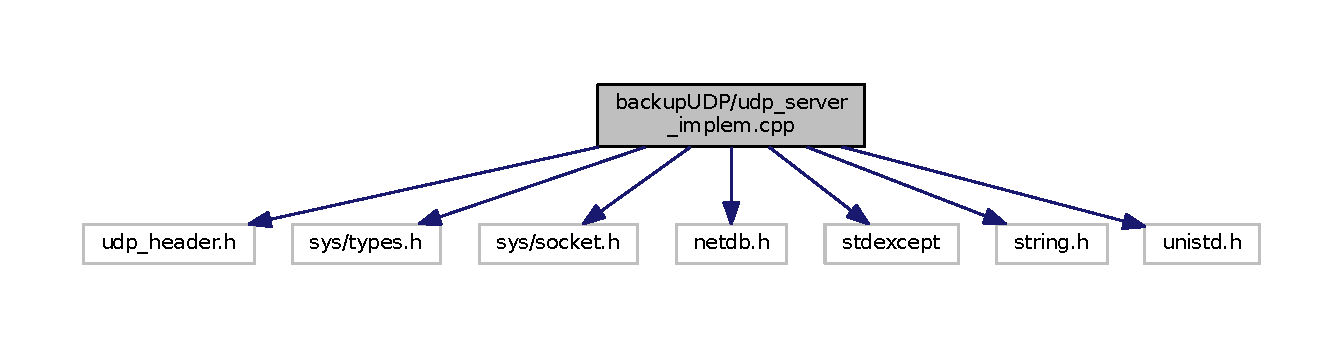
\includegraphics[width=350pt]{udp__server__implem_8cpp__incl}
\end{center}
\end{figure}
\subsection*{Namespaces}
\begin{DoxyCompactItemize}
\item 
 \hyperlink{namespaceudp__client__server}{udp\+\_\+client\+\_\+server}
\end{DoxyCompactItemize}

%--- End generated contents ---

% Index
\backmatter
\newpage
\phantomsection
\clearemptydoublepage
\addcontentsline{toc}{chapter}{Index}
\printindex

\end{document}
